\chapter{Methodology}

\section{Short-Time Fourier Transform}
For a piece of music typically exhibits a recurring structure characterized by continuous variation over time, hence it is extremely difficult to classify the process of musical audio data as stationary, whether in the strict or weak sense. In strict stationarity, all components of the processes must remain invariant under time shifts, whereas in weak stationarity, it suffices for only the first moments (means) and second moments (such as variances and covariances) to be invariant over time. However, almost all music involves dynamic changes in rhythm, melody, harmony, and instrumentation, which cause fluctuations in the underlying statistical properties of the audio data.\\
\\
We may consider the song L'anno che verrà as an example, which was composed by the well-known Bolognese musician Lucio Dalla. The audio file used in this case has a sampling rate of 44.1 kHz, which is a standard rate for high-quality audio recordings. This means that the waveform is represented by 44,100 data points per second, resulting in a high-resolution time series. By inspecting the waveform plot shown in Figure \ref{fig:L'anno che verrà}, it becomes apparent that the audio signal does not exhibit constant variance or covariance over time. In other words, the statistical properties of the signal appear to change throughout the recording. Visually, one can find fluctuations in amplitude that suggest non-stationary behavior. Although this observation is made somewhat intuitively from the graph, it gives a preliminary indication that treating the audio signal as a stationary process would not be appropriate.\\
\begin{figure}[H]
	\centering
	\includegraphics[width=0.9\linewidth]{../Statistical_Sciences_template/figure/Waveform.png}
	\caption{Time-domain waveform of L'anno che verrà from 15s to 75s, showing amplitude variations over time. The horizontal axis represents time in seconds, while the vertical axis shows normalized amplitude. If we reckon the waveform audio signal as a time series, we can intuitively say the process is heteroschedastistic and non-stationary.}
	\label{fig:L'anno che verrà}
\end{figure}
\noindent To address the challenge of non-stationary audio signals, a typical and widely adopted strategy is the application of the Short-Time Fourier Transform (STFT). The fundamental assumption behind STFT is that, although the overall audio signal is non-stationary, it can be considered approximately stationary in short time frames. Within these frames, it is assumed that the spectral characteristics of the signal are approximately constant. In practice, the audio data is segmented into partially overlapping short frames, and for each frame, the Discrete Fourier Transform (DFT) is computed. The steps can be conclude in the following way:\\
\\
\usetikzlibrary{arrows.meta}
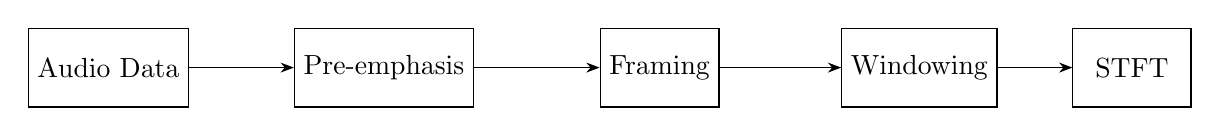
\begin{tikzpicture}[->, >=Stealth]
	
	\node[draw, rectangle, minimum width=1.5cm, minimum height=1cm] (A) at (-4.5,0) {Audio Data};
	\node[draw, rectangle, minimum width=1.5cm, minimum height=1cm] (B) at (-1,0) {Pre-emphasis};
	\node[draw, rectangle, minimum width=1.5cm, minimum height=1cm] (C) at (2.5,0) {Framing};
	\node[draw, rectangle, minimum width=1.5cm, minimum height=1cm] (D) at (5.8,0) {Windowing};
	\node[draw, rectangle, minimum width=1.5cm, minimum height=1cm] (E) at (8.5,0) {STFT};	
	
	\draw (A) -> (B);
	\draw (B) -> (C);
	\draw (C) -> (D);
	\draw (D) -> (E);	
\end{tikzpicture}
\\
\section{Mel Scale}

The invention of the Mel scale can be traced back to 1937, as previously mentioned in the introduction. The idea behind it originated from psychological studies in the field of psychology, specifically investigating the non-linear nature of human auditory perception. In their pioneering work, Stevens, Volkmann, and Newman established the foundation of the Mel scale through experimental research demonstrating that the human ear exhibits greater sensitivity to changes in low-frequency sounds and reduced sensitivity at higher frequencies. This means that small changes in low-frequency sounds are more easily perceived than equivalent changes in high-frequency sounds. In the same way it also indicated that the perception of pitch by the human auditory system does not follow a linear relationship with physical frequency. The data from their experiments showed that the relationship between physical frequency (in Hertz) and perceived pitch (in Mels) is non-linear, resembling the shape of an exponential function rather than a straight line. Unfortunately they didn't provide any mathematical formula to describe this phenomenon. Later researchers, building on the foundational experimental data, designed a mathematical model to describe this non-linear relationship more precisely and wildly used today:\\
\begin{equation}
   Mel(f)=2595\log_{10}(1+\frac{f}{700}) \label{Mel Scale}
\end{equation}
where $Mel(f)$ is the Mel scale and $f$ is the frequency. Thus for the convenience of computing, using the base changing formula for logarithm we can get the equivalent one, the formula can be represented in the following way: \\
\begin{equation}
   Mel(f)=1127\ln(1+\frac{f}{700})
\end{equation}
Via these formulas we can transform the nonlinear human pitch perception into a computable linear scale.\\
\\

\section{Mel Frequency Cepstral Coefficients}

The Mel Frequency Cepstral Coefficients (MFCCs) are a widely used feature representation in audio signal processing, particularly effective in tasks such as music genre classification. The computation of MFCCs is fundamentally based on two key components: the Short-Time Fourier Transform (STFT) and the Mel scale. STFT provides a time-frequency representation of the audio signal, capturing its spectral characteristics within short, overlapping frames, while the Mel scale transforms the linear frequency axis into a perceptually motivated scale. The steps are illustrated in the following diagram, which outlines the complete pipeline for MFCC extraction.
\\

\usetikzlibrary{arrows.meta}
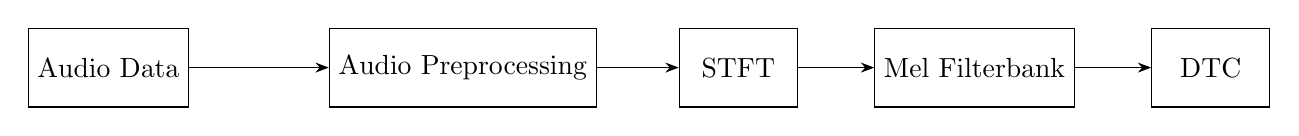
\begin{tikzpicture}[->, >=Stealth]

	\node[draw, rectangle, minimum width=1.5cm, minimum height=1cm] (A) at (-4.5,0) {Audio Data};
	\node[draw, rectangle, minimum width=1.5cm, minimum height=1cm] (B) at (0,0) {Audio Preprocessing};
	\node[draw, rectangle, minimum width=1.5cm, minimum height=1cm] (C) at (3.5,0) {STFT};
	\node[draw, rectangle, minimum width=1.5cm, minimum height=1cm] (D) at (6.5,0) {Mel Filterbank};
	\node[draw, rectangle, minimum width=1.5cm, minimum height=1cm] (E) at (9.5,0) {DTC};	
	
	\draw (A) -> (B);
	\draw (B) -> (C);
	\draw (C) -> (D);
	\draw (D) -> (E);	
\end{tikzpicture}
\\
\\
To provide a clearer understanding of the process above for computing MFCCs, it is helpful to break it down step by step.\\
\subsection{Pre-emphasis}
The first step in the MFCC extraction pipeline is pre-emphasis, a preprocessing operation applied to the raw audio signal. The purpose of pre-emphasis is to amplify the high-frequency components of the signal, which are often attenuated during the sound production or transmission process. This step not only improves the spectral balance but also enhances the signal-to-noise ratio for high-frequency elements. Typically, a first-order high-pass filter is employed for pre-emphasis. This filter is simple yet effective and is commonly defined in the time domain by the equation:\\
\begin{equation}
y(t)=x(t)-\alpha x(t-1) \label{pre-emphasis}
\end{equation}

in which $x(t)$ is the input signal, $y(t)$ is the filtered output and  $\alpha$  is the pre-emphasis coefficient, usually chosen in the range of 0.95 to 0.97.In the Z-domain, which is frequently used in digital signal processing for system analysis, the corresponding transfer function of the high-pass filter is:\\
\begin{equation}
H(t)=\frac{Y(z)}{X(x)}=1-\alpha z^{-1}
\end{equation}
where $X(z)=\sum_{t=-\infty}^{\infty}x(t)z^{-t}$ that represents the Z-transform of the input signal and $z$ is complex variable that $z^{-1}$ is the one-step delay operator. The input spectrum multiplied by the transfer function of the high-pass filter is the output spectrum. This spectral filtering emphasizes the higher frequency regions, preparing the signal for subsequent stages. \\
\subsection{Framing and Windowing} \label{subsec:framingwindowing}
The second step is framing and windowing, which prepare the audio signal for localized frequency analysis in the time-frequency domain. In the framing step, the pre-emphasized audio signal is split into short frames that are overlapping with each other, under the assumption that the signal is approximately stationary within each frame. This is a practical simplification, as real-world audio signals——such as speech and music——are always non-stationary, both in the strict and weak statistical sense, as I have illustrated in the first section of this chapter. Hence frames help for a more accurate and localized spectral analysis. For the m-th frame, the signal segment can be defined as:\\
\begin{equation}
y_m[t]=y[t+m\times h], \qquad 0\leq t<L \label{framing}
\end{equation}
where $y(t)$ is the pre-emphasized signal from \eqref{pre-emphasis}, $L$ is the frame length and $h$ is the hop size which determines the step between consecutive frames and controls the degree of overlap.
Following framing, a window function is applied to each frame to reduce spectral leakage—a phenomenon that arises due to the finite length of frames, which can introduce discontinuities at the boundaries and distort the spectral representation. To mitigate this, each frame is multiplied element-wise by a tapering function that smooths the edges. Two commonly used window functions are the Hamming window and the Hann window, defined respectively as:\\
  Hamming:
  \begin{equation}
  w[t]=0.54-0.46\cos(\frac{2\pi n}{L-1}) \label{Hamming}
  \end{equation}
  Hann:
  \begin{equation}
  w[t]=0.5-0.5\cos(\frac{2\pi n}{L-1}) \label{Hann}
  \end{equation}
The windowed frame is then computed by multiplying the framed signal by the window function:\\
\begin{equation}
	y_{win}[t]=y_m[t]\times w[t] \label{windowing}
\end{equation}
\subsection{Short-Time Fourier Transformation}
The third step is to perform Fourier transformation on each frame of signal. This transformation converts the time-domain signal into its frequency-domain representation, yielding a complex-valued spectrum for each frame, that is $X_m[k]$ where $k$ is the frequency bin index. The discrete Fourier Transform (DFT) of a windowed signal frame can be computed as follows:\\
\begin{equation}
X_m[k]=\sum_{t=0}^{L-1}y_{win}[t]\times e{\frac{-2\pi kti}{N}} \label{DFT}
\end{equation}
where i represents the imaginary unit satisfying $i^2=-1$, $N$ is DFT size and k is the frequency bin index.\\
\\
The results of $X_m[k]$ are complex numbers representing the magnitude and phase of the frequency component at bin $k$ for frame $m$. However, for most MFCC applications, only the magnitude or power spectrum are used, discarding the phase information. To obtain the amplitude spectrum, we compute the modulus of the complex DFT coefficients: \\
\begin{equation}
|X_m[k]|=\sqrt{Real(X_m[k])^2+Imag(X_m[k])^2}
\end{equation} 
Alternatively, the power spectrum can be obtained by squaring the amplitude:
\begin{equation}
|X_m[k]|^2=Real(X_m[k])^2+Imag(X_m[k])^2
\end{equation}
This step provides a frequency-based representation of each frame that captures how energy is distributed across frequency bands. The $k\times m$ matrix of power spectra (more popular) is then passed to the Mel filter bank in the next step to simulate the human auditory system’s nonlinear frequency resolution.\\
\subsection{Mel Filter Bank}
Hence the fourth step is the construction of the Mel filter bank, which plays a key role in modeling the human auditory system’s nonlinear perception of frequency. The Mel filter bank is composed of a set of overlapping triangular filters that are spaced linearly on the Mel scale but non-linearly on the Hertz (Hz) scale.\\
\\
The first consideration in designing the Mel filter bank is to determine the frequency range. Typically, this range should cover the entire audible frequency spectrum for humans, which is approximately 20 Hz to 20,000 Hz. However, in practice, the upper bound is often constrained by the Nyquist frequency, which is half the sampling rate of the audio signal. For example, if the sampling rate is 22050 Hz, the Mel filter bank will be designed from 0 Hz to 11025 Hz.\\
\\
Once the frequency range in Hz is determined, the next step is to map these boundaries to the Mel scale using \eqref{Mel Scale}. Specifically, we compute:
\begin{equation}
Mel_{min}=Mel(0), \qquad  Mel_{max}=Mel(f_{max})
\end{equation}
where $f_max=\frac{sampling rate}{2}$ mentioned above.\\
\\
Next, we decide on the number of filters, denoted by $\nu$, which determines the frequency resolution in the perceptual domain. Based on this, we partition the Mel scale uniformly into $\nu+2$ points, corresponding to the lower edge, center, and upper edge frequencies of each triangular filter. These center Mel frequencies are spaced across the interval $[Mel_{min}, Mel_{max}]$. After obtaining these center points on Mel scale, we can convert them back to the form of Hertz using the inverse formula of \eqref{Mel Scale}, that is: \\
\begin{equation}
f=700\times (10^{\frac{Mel}{2595}}-1)
\end{equation}\\
Once the center frequencies have been determined and mapped back to the Hertz domain, the next step is to construct the triangular Mel filters.These filters are designed to mimic the frequency resolution of the human ear by emphasizing specific frequency bands and smoothing transitions between adjacent bands. As previously noted, the filters are overlapping and each has a triangular shape with values ranging from 0 to 1. For example, the $\kappa$-th filter denoted as $H_{\kappa}(f)$ is defined over the interval $[f_{\kappa-1},f_{\kappa+1}]$ where $f_{\kappa-1}$, $f_{\kappa}$ and $f_{\kappa+1}$ are the lower boundary, center frequency, and upper boundary of the filter in Hertz domain respectively. The filter starts with a value of 0 at $f_{\kappa-1}$, increases linearly to a peak value of 1 at the center point $f_{\kappa}$, and then decreases linearly back to 0 at $f_{\kappa+1}$.  Mathematically, this can be expressed as:\\
\begin{equation}
H_{\kappa}(f)=
\begin{cases}
	0  & f<f_{\kappa-1}\\
	\frac{f-f_{\kappa-1}}{f_{\kappa}-f_{\kappa-1}}  & f_{\kappa-1}\leq f<f_{\kappa} \\
	\frac{f_{\kappa+1}-f}{f_{\kappa+1}-f_{\kappa}}  & f_{\kappa}\leq f<f_{\kappa+1} \\
	0  & f \geq f_{\kappa+1}
\end{cases}	
\end{equation}
Each filter effectively weights the STFT spectrum based on how close a frequency component is to the filter's center frequency. This construction ensures that each frequency bin contributes to multiple filters, allowing the system to capture smooth transitions and localized energy in neighboring frequency bands. The overlapping nature of the filters also reflects the way human auditory perception blends adjacent frequencies rather than treating them as completely distinct.\\
\\
Figure~\ref{fig:Mel filters} illustrates an example of a Mel filter bank spanning the frequency range from 0 to 11025 Hz, constructed with 10 triangular filters. In the figure, the red triangle represents the $\kappa$-th filter $H_{\kappa}(f)$, while the blue and green triangles correspond to the adjacent filters $H_{\kappa-1}(f)$ and $H_{\kappa+1}(f)$ respectively. As shown, the filters are overlapping, with each one peaking at its center frequency and tapering linearly to zero at the boundaries shared with neighboring filters. The widths of the triangles vary, reflecting the non-linear spacing of Mel-scale frequencies when mapped back to the linear Hertz scale. But in practice, especially in analysis of music we will design more Mel filters for weighting the results of the STFT matrix.\\
\begin{figure}
	\centering
	\includegraphics[width=0.9\linewidth]{../Statistical_Sciences_template/figure/example of Mel filters.png}
	\caption{}
	\label{fig:Mel filters}
\end{figure}\\
After constructing the Mel filter bank, the next step is to compute the Mel-scale energy coefficients, which represent the energy content of the signal in perceptually motivated frequency bands. This step effectively transforms the detailed frequency representation obtained from the power spectrum into a compact and interpretable form aligned with the Mel scale. The computation consists of two primary stages. First, the power spectrum $|X_m[k](f)|^2$ of each frame (as derived from the STFT) is weighted by the Mel filter bank. For each Mel filter $H_{\kappa}$, the power spectrum is multiplied point-wise by the filter’s response across frequencies.Next, the weighted values are summed to obtain the total energy within each Mel frequency band. This aggregation yields the Mel energy coefficient for the $\kappa$-th filter, which can be expressed mathematically as:\\
\begin{equation}
Mel_{\kappa}=\sum_{f} |X_m[k](f)|^2 \times H_{\kappa}(f)
\end{equation}
where $Mel_{\kappa}$ is the energy in the $\kappa$-th Mel band for the m-th frame.\\ 
\\
The final step of this part is to do logarithm compression for the Mel scale energy coefficients. The purpose of this operation is to compress the dynamic range of Mel energies enhancing low-amplitude components while taming high-amplitude peaks. In this compression we must choose a small constant denoted as $\epsilon>0$ to avoid computing $\log(0)$ and then compute the log-Mel spectrum within $\log(Mel_{\kappa}+\epsilon)$. Finally denoting the number of Mel scale energy coefficients as $\nu_{mel}$, we can get a $\nu_{mel} \times m$ matrix.\\
\subsection{Discrete Cosine Transform}
The final stage in computing Mel Frequency Cepstral Coefficients (MFCCs) is to apply the Discrete Cosine Transform (DCT) to the log-transformed Mel energy coefficients. This step serves two primary purposes: first, it decorrelates the log-Mel energies, making the resulting features approximately orthogonal and hence more suitable for statistical modeling; second, it helps to separate the spectral envelope (which carries information about the timbre of the sound) from the excitation signal (which often corresponds to pitch or voiced/unvoiced characteristics). More specifically, the DCT Type-II is typically applied, which transforms the logarithmic Mel spectrum into the cepstral domain. The transformation is defined as follows:\\
\begin{equation}
	MFCC_n=\sum_{\kappa=1}^{\nu_{mel}}[\log(Mel_{\kappa})\times \cos(\frac{n(\kappa-0.5)\pi}{\nu_{mel}})]
\end{equation}
where $n$ is the index of the cepstral coefficients and $MFCC_n$ is the $n$-th Mel frequency cepstral coefficient. Typically $n$ ranges from 0 to 12 or 13, but in some situations more will be taken. Finally we got a $n \times m$ matrix.\\
\\
By concentrating most of the signal energy in the lower-order coefficients, the DCT facilitates dimensionality reduction and helps isolate perceptually significant information. In practice, only the first few MFCCs are retained, as they capture the most relevant features of the audio signal's spectral shape, while higher-order coefficients are often discarded or used selectively depending on the application.\\
\subsection{An Example of MFCC}

To illustrate the process concretely, I also take L'anno che verrà as an example. The audio file used in this example has a standard sampling rate of 44.1 kHz, as mentioned in the first section of this chapter. For the purposes of analysis, I selected a 60-second excerpt beginning at the 15-second mark. In preparing the signal for time-frequency analysis, I chose a window size (also referred to as the frame length) of 1024 samples. This corresponds to a segment of the audio that spans:\\
$$
	\frac{1024}{44100}\approx0.0232 \ \text{seconds} \qquad \text{(or approximately 23 milliseconds)}
$$
It is worth noting that this duration is significantly shorter than a full second, as one-second windows typically capture too much variation in dynamic audio signals, making it difficult to assume any form of stationarity within them.\\
To allow for continuity and smoother temporal analysis, a hop size of 256 samples was used, which is exactly one-quarter of the window size. This means that each analysis window overlaps 0.75 with the next. The hop duration in time can be calculated as:\\
$$
	\frac{256}{44100}\approx0.0058 \ \text{seconds} \qquad \text{(or approximately 5.8 milliseconds)}
$$
After framing and windowing, MFCCs are computed per frame. For this example, I selected the standard 13 MFCCs ($n=13$) per frame, which is a commonly used configuration in audio analysis as it strikes a balance between capturing relevant spectral features and avoiding redundancy. The output of the MFCC process is a matrix of size $n \times m$, where $m$ represents the total number of frames computed for the audio segment.\\
\\
The total number of frames $m$ is calculated by the following formula
\begin{equation}
	number\textunderscore of\textunderscore frames=\lceil \frac{sample\textunderscore rate \times duration-frame \textunderscore length}{hop\textunderscore length}+1 \rceil
	\label{windownumber}
\end{equation}\\
In our situation:
\begin{itemize}
	\item $\text{sample\_rate} = 44100$,
	\item $\text{duration} = 60$ seconds,
	\item $\text{frame\_length} = 1024$, and
	\item $\text{hop\_length} = 256$.
\end{itemize}
Hence substitute the values we can get:\\
$$
number\textunderscore of\textunderscore frames=\lceil \frac{44100*60-1024}{256}+1\rceil=10333
$$\\
Therefore, the resulting MFCC matrix has dimensions $13\times 10333$.\\
\\
The following figure \ref{fig:MFCC Example} is the MFCC spectogram of the piece of music. For the $y$ axis it is divided into 13 intervals that corresponds to the 13 MFCCs. Thus the $x$ axis various over time from 0s to 60s, hence the figure illustrate how energy distribution during the time. For example, the high-order MFCCs are almost uniformly distributed from 30s to 40s. It is possible that some instruments are playing continuously, making the energy change less obvious, while there is a significant energy changes from 25s to 30s. \\
\\
\begin{figure}
	\centering
	\includegraphics[width=0.9\linewidth]{../Statistical_Sciences_template/figure/MFCC Example.png}
	\caption{}
	\label{fig:MFCC Example}
\end{figure}\\
The first few MFCCs (such as the 1st to 3rd dimensions) mainly capture the characteristics of the vocal tract (low-frequency cepstrum components). These coefficients reflect the spectral envelope characteristics of the sound, especially the resonance peak structure that is closely related to the shape of the vocal tract. Since the vocal tract changes relatively slowly (such as the movement of the vocal organs takes a certain amount of time), as shown in figure \ref{fig:Low MFCCs}, these low MFCCs appear as curves in the time domain that do not change particularly drastically, but the difference is significant.\\
\\
\begin{figure}[h!]
	\centering
	\includegraphics[width=0.9\linewidth]{../Statistical_Sciences_template/figure/Low MFCCs.png}
	\caption{}
	\label{fig:Low MFCCs}
\end{figure}\\
However, high-order MFCCs (such as the 11th-13th dimension and above) mainly reflect the detailed characteristics of the excitation source (high-frequency cepstrum components). These coefficients record the finer time-varying characteristics of the sound signal. Since the characteristics of the excitation source (such as the fundamental frequency generated by the vibration of the vocal cords or the random noise of the unvoiced sound) often have rapidly changing transient characteristics, they are manifested as violent fluctuations in the high-frequency coefficient curve in the MFCC spectrogram as shown in figure \ref{fig:High MFCCs}. This fluctuation pattern is directly related to the excitation characteristics of the sound. It is worth noting that high-order MFCC coefficients often show a high degree of similarity. This is because in these cases, the characteristics of the excitation source (such as the vocal cord vibration mode or the noise characteristics) remain relatively constant, and the changes mainly occur in the vocal tract characteristics.\\
\begin{figure}[h!]
	\centering
	\includegraphics[width=0.9\linewidth]{../Statistical_Sciences_template/figure/High MFCCs.png}
	\caption{}
	\label{fig:High MFCCs}
\end{figure}\\

\section{Shapelet Tree-Based Classification}

This algorithm is inspired by the foundational work of L. Ye and E. Keogh (2009), which introduced a novel approach for time series classification based on the concept of shapelets. A shapelet is defined as a subsequence of a time series that is maximally representative of a particular class. In other words, a shapelet captures a discriminative pattern or local structure that tends to appear in time series belonging to one class but not in others. The primary objective of the algorithm is to identify the most informative shapelet——i.e. the one that best separates the classes. This is typically achieved by evaluating candidate subsequences based on their ability to split the dataset according to a distance threshold, using measures such as information gain to quantify the separation.\\
\\
Once the optimal shapelet has been discovered, it can be used to transform the time series into a new feature space where each instance is represented by its distance to the shapelet(s). This transformation enables the application of traditional classification techniques such as decision trees, as the complex temporal data are now reduced to a more tractable feature-based representation. The shapelet-based approach provides both interpretability, as the identified shapelets can be visualized and interpreted as the key patterns driving the classification. This makes the algorithm particularly valuable in domains where understanding the decision process is important.\\
\subsection{Key Definitions}
Before delving into the details of the algorithm, it is essential to introduce several key definitions that form the theoretical foundation for understanding the overall process. These definitions help clarify the notions of distance between time series and provide a framework for comparing sequences of potentially different lengths.
\begin{definition}[Distance of time series with the same length]%
Let $Dist(T_1,T_2)$ denote the distance between two discrete time series $T_1$ and $T_2$, where $T_1$ and $T_2$ are two discrete time series who may have the same length. A valid distance function must satisfy the following properties:\\
1. Symmetry: $Dist(T_1,T_2)=Dist(T_2,T_1)$ and \\
2. Non-negativity: $Dist(T_1,T_2) \geq 0$. 
\end{definition}%
\noindent For example, if we compute the Euclidean distance between $T_1$ and $T_2$, the formula follows:
$$
Dist(T_1,T_2)=(\sum_i(T_{1i}-T_{2i})^2)^{\frac{1}{2}}
$$
Alternatively, the Manhattan distance can be used:\\
$$
Dist(T_1,T_2)=\sum_i|T_{1i}-T_{2i}|
$$
In practical applications, it is more common to encounter the cases that two time series do not have equal lengths, i.e., $length(T_1^*) \neq length(T_2^*)$. Without lose generality, we can assume $length(T_1^*)\geq length(T_2^*)$. In such cases, we consider the distance between the two time series is based on the best matching subsequence of the longer series $T_1^*$. Hence the distance between $T_1^*$ and $T_2^*$ can be define as:

\begin{definition}[Distance of time series]\label{def:Dist}%
$Dist(T_1^*,T_2^*)=\min_{S\subseteq T_1^*}(Dist(S,T_2^*))$ where $S$ is a subsequence of $T_1^*$ having the same length as $T_2^*$ 
\end{definition}%
\noindent Another key concept in this algorithm is the notion of a shapelet, which can be described as follows:
\begin{definition}[Shapelet]\label{def:shapelet}%
	Give a labeled time series dataset $\boldsymbol{D}$ which contains two classes of observations, denoted as $A$ and $B$, shapelet($\boldsymbol{D}$) is defined as a subsquence of a time series within $\boldsymbol{D}$ that best separates the observations according to their class labels.
\end{definition}%
\noindent In other words, a shapelet is a short, discriminative segment of a time series that captures distinctive features associated with one class and is absent or significantly different in the other. The fundamental idea behind using shapelets is that certain local patterns, rather than the entire time series, can be highly informative for classification. Once a candidate shapelet has been extracted, the algorithm evaluates its usefulness by assessing how well it partitions the dataset based on similarity to the shapelet. Moreover to evaluate how well a given subsequence (i.e., a shapelet candidate) can partition the dataset according to the class labels, this algorithm uses information gain (IG) as the primary quality metric. Information gain measures the reduction in uncertainty (entropy) about class membership after the dataset has been split based on the shapelet. It can be calculated as:\\
\begin{equation}
	IG=I(\boldsymbol{D})-f(\boldsymbol{D_1})\times I(\boldsymbol{D_1})-f(\boldsymbol{D_2})\times I(\boldsymbol{D_2})
	\label{IG}
\end{equation}
where $I(\boldsymbol{D})$ denotes the entropy of the original dataset $\boldsymbol{D}$, while $I(\boldsymbol{D_1})$ and $I(\boldsymbol{D_2})$ are the entropies of the two subsets resulting from a split based on a candidate shapelet. ,$f(D_i) \forall i=1,2$ represent the proportion of observations of $D_1$ and $D_2$ in $D$ respectively.\\
\\
By using formula \eqref{IG}, we can compute the information gain of each split datasets $D_1$ and $D_2$, and we can choose the best sequence that gives the largest information gain as the shapelet. Hence only one problem is remained that is how the shapelet can classify the time series datasets and find the best split point that corresponds to the shapelet. Here follows another definition of vital importance:
\begin{definition}[Optimal Split Point]
Given a time series dataset $\boldsymbol{D}$ consisting of two classes $A$ and $B$, for a shapelet candidate $S$, we can choose a distance threshold $d_{th}$ splitting $\boldsymbol{D}$ into two subsets $\boldsymbol{D_1}$ and $\boldsymbol{D_2}$ whose intersection is empty, i.e. $\boldsymbol{D_1} \cap \boldsymbol{D_2}=\emptyset$, such that $\{T_i, Dist(T_i,s)\leq d_{th} \forall T_i \in \boldsymbol{D} \}$ are assigned to one class and $\{T_i, Dist(T_i,s) > d_{th} \forall T_i \in \boldsymbol{D} \}$ are assigned to the other class. Thus the optimal split point (OSP) is the threshold that 
$$
	IG(S, d_{OSP}) \geq IG(S, d_{th})
$$
In other words, the OSP is the threshold that:\\
$$
	d_{OSP}=\arg \max_{d_{th}} IG (S,d_{th})
$$
\label{def:OSP}
\end{definition}

\begin{figure}[h!]
	\centering
	\includegraphics[width=0.9\linewidth]{../Statistical_Sciences_template/figure/OSP.png}
	\caption{There are 13 observations in the dataset, they are shown via the distances of candidate shapelet $S$, and the shapes corresponds to different labels. The optimal split point is the center point between the 7th sorted observation and the 8th sorted observation}
	\label{fig:OSP}
\end{figure}

\noindent To illustrate the concept of the optimal split point, we can refer to the Figure \ref{fig:OSP}. The process begins by computing the distance between a candidate shapelet $S$ that is a subsequence of one time series from $\boldsymbol{D}$ and all the times series in dataset $D$. If the dataset $D$ contains $n$ observations we will obtain $n$ distance values. Because each time series in the dataset is labeled, we can sort the distances in ascending order and associate them with their corresponding class labels. Using this sorted list, we iterate over all possible split points between consecutive distances and calculate the entropy of the resulting subsets for each threshold. The information gain is computed for each potential split using Equation \eqref{IG}, and the threshold that results in the highest information gain is selected as the optimal split point.\\
\\
This approach allows the algorithm to determine both the most discriminative shapelet and the decision boundary (distance threshold) that best separates the classes, forming the basis for subsequent classification of new time series based on their similarity to the learned shapelet.\\
\\
\subsection{Achieve of the Shapelet Algorithm}\label{sec:algo}

To implement the shapelet-based classification algorithm, the first and most crucial step is to generate all possible shapelet candidates $S$ from the given time series dataset $D$ referring to Definition \ref{def:shapelet}. In practice, shapelet candidates are formed by extracting all possible contiguous subsequences from the time series instances in $D$. Hence the generating step can be achieve as follows:\\
\begin{algorithm}[h!]
	\caption{Candidate Shapelets Generating}
	\begin{algorithmic}[1]{
		\Procedure{generate\ candidates}{$\mathtt{Time\ Series}\ T$, $MINLEN$, $MAXLEN$}
		\State $pool \gets \emptyset$
		\State $l \gets MAXLEN$
		\While{$l \geq MINLEN$}{
			\For{$i \gets 1$ \textbf{to} $\mathrm{len}(T) - l$}
			\State \textbf{EXTRACT subsequence from T starting at i with length l} 
			\State \textbf{ADD subsequence to pool} 
			\EndFor
		}
		\State $l \gets l - 1$
		\EndWhile
		\EndProcedure
	}
	\end{algorithmic}
	\label{al:CandidateGenerate}
\end{algorithm}
\\
As mentioned above, this function is designed to generate the complete set of consecutive subsequence candidates from a given time series sequence $T$ where the lengths of the subsequences range from a specified minimum length $MINLEN$ to a maximum length $MAXLEN$. The goal is to produce all possible contiguous segments of $T$ that fall within this length interval, which will later be evaluated for their usefulness as shapelets.\\
\\
The implementation follows a nested loop structure:
\begin{quote}
1. The outer loop iterates over the possible subsequence lengths l, starting from $MAXLEN$ and decrementing down to $MINLEN$. This ordering ensures that longer subsequences are generated and added to the pool before the shorter ones.\\
\\
2. For each fixed length $l$, the inner loop performs a sliding window operation across the sequence $T$. It moves a window of length 
$l$ one step at a time (i.e., with a stride of 1), starting at every valid index $i$ such that the subsequence $T[i:i+1]$ emains within bounds.
\end{quote}
Each generated subsequence is stored in the candidate pool. This format facilitates efficient indexing and retrieval in later stages of the algorithm, particularly when computing distances and information gain. The final output of the function is a list containing all valid subsequences from T whose lengths fall within the defined range. The resulting pool is ordered from longest to shortest subsequences, reflecting the traversal logic described above.\\
\\
After obtaining the complete set of candidate subsequences—also known as shapelet candidates—the next critical step is to compute the distances between each shapelet and all time series in the dataset referring to Definition \ref{def:Dist}. This involves sliding each shapelet across every time series and calculating the minimum distance between the shapelet and the most similar subsequence within each series. The algorithm can be achieve as follows:\\
\begin{algorithm}[H]
	\caption{Time Series Distance}
	\begin{algorithmic}[1]{
			\Procedure{subsequence\ dist}{$\mathtt{Time\ Series}\ T$, $\mathtt{Time\ Series}\ S$, $metric$}
			\State $len \textunderscore T \gets \mathtt{LENGTH\ of}\ T$
			\State $len \textunderscore S \gets \mathtt{LENGTH\ of}\ S$
			\State $min \textunderscore dist \gets +\infty$
			\For{$i \gets 1$ \textbf{to} $(len \textunderscore T - len \textunderscore S)$}
			\State $window \gets T[i:\ i + len \textunderscore S]$
			\State $dist \gets Dist(window,S)$ 
			\If {$dist< min \textunderscore dist$}
			\State $min \textunderscore dist \gets dist$ 
			\EndIf
			\EndFor
			\EndProcedure
		}
	\end{algorithmic}
	\label{al:DIST}
\end{algorithm}

\noindent This function calculates the distance of the subsequence most similar to the target sequence S in the sequence T, and controls the measurement methods of distance through the variable metric, such as two measurements: Euclidean and Manhattan distance (L1). Iterate through the sliding window all subsequences of length $len(S)$ in $T$. For each window, calculate its distance from $S$ according to the specified metric: if it is the Euclidean distance, calculate the sum of the squared difference; if it is the Manhattan distance, calculate the sum of the absolute difference. Finally, the minimum value of all window distances is returned.\\
\\
Next, using the distances computed in the previous step, the algorithm proceeds to identify the optimal split point. As outlined in the previous section and formally defined in Definition \ref{def:OSP}, this step is crucial for evaluating how effectively a shapelet can separate the time series into distinct classes. The process begins by sorting the computed distances between a candidate shapelet and all time series in ascending order. This sorted list enables us to systematically examine potential thresholds for splitting the dataset. Once the distances are sorted, a distance-based histogram is constructed, where each bin corresponds to a range of distances, and each time series is assigned a class label. The algorithm goes as follows:\\
\begin{algorithm}[H]
	\caption{Check Candidate}
	\begin{algorithmic}[1]{
			\Procedure{checkcandidate}{$\boldsymbol{D}$, $S$, $original\textunderscore label$}
			\State $object_histogram \gets \emptyset$
			\For{$\mathtt{EACH}\ T$ \textbf{in} $\mathtt{Dataset}\ \boldsymbol{D}$}
			\State $dist \gets SUBSEQUENCEDIST(T,S)$
			\State \textbf{ADD dist to} $object_histogram$
			\EndFor
			\State \textbf{RETURN CalculateInformationGain}$(object\textunderscore histogram, original\textunderscore label)$
			\EndProcedure
		}
	\end{algorithmic}
	\label{al:checkcandidate}
\end{algorithm}
\noindent The purpose of this function is threefold: (1) calculate the minimum distance between the candidate shapelet $S$ and every sequence in the dataset $D$ using a specified distance metric, (2) compile a histogram of these distances, and (3) compute the information gain associated with the best possible split based on these distances.\\
\\
The specific process unfolds as follows:
\begin{quote}
1. Iterate over each time series $T$ in the dataset $\boldsymbol{D}$. For each sequence, the function invokes SUBSEQUENCEDIST referring the Algorithm \ref{al:DIST}, which calculates the distance between $S$ and $T$, using the chosen metric (e.g., Euclidean or Manhattan distance). This results in a single scalar value representing how closely $T$ matches $S$.\\
2. Each computed distance is then stored in a list called object\textunderscore histogram, which contains the distance values. \\
3. The histogram and original class labels are passed to the CalculateInformationGain function.
\end{quote}

\noindent But in the Algorithm \ref{al:checkcandidate} there is another function to be used, that is CalculateInformationGain, which aims at finding the optimal split of the input shapelet, calculating the information gain and split the time series dataset $\boldsymbol{D}$ into two $\boldsymbol{D_1}$ and $\boldsymbol{D_2}$. To complete this function the algorithm follows:
\begin{algorithm}[H]
	\caption{Calculate Information Gain}
	\begin{algorithmic}[1]{
			\Procedure{CalculateInformationGain}{$object\textunderscore histogram$, $original\textunderscore label$}
			\State $key \gets \mathtt{Empty\ dictionary}$
			\State $\boldsymbol{D_1} \gets \emptyset$
			\State $\boldsymbol{D_2} \gets \emptyset$
			\State $split\textunderscore 	point \gets$ \textbf{OptimalSplitPoint}($object\textunderscore histogram$, $original\textunderscore label$)
			\For{$d$ \textbf{in} $object\textunderscore histogram$}
			\If{$d \leq split_point$}
			\State $\boldsymbol{D_1} \gets \boldsymbol{D_1} \bigcup d$ 
			\Else $\boldsymbol{D_2} \gets \boldsymbol{D_2} \bigcup d$ 
			\EndIf
			\EndFor	
			\State $Entropy_{\boldsymbol{D}} \gets ENTROPY(\boldsymbol{D})$
			\State $Entropy_{\boldsymbol{D_1}} \gets ENTROPY(\boldsymbol{D_1})$
			\State $Entropy_{\boldsymbol{D_2}} \gets ENTROPY(\boldsymbol{D_2})$
			\State $Proportion_{\boldsymbol{D_1}} \gets PROPORTION(\boldsymbol{D_1})$
			\State $Proportion_{\boldsymbol{D_2}} \gets PROPORTION(\boldsymbol{D_2})$
			\State $IG \gets Entropy_{\boldsymbol{D}}-(Proportion_{\boldsymbol{D_1}} \times Entropy_{\boldsymbol{D_1}}+Proportion_{\boldsymbol{D_2}} \times Entropy_{\boldsymbol{D_2}})$
			\State \textbf{Store} $split\textunderscore point$, $IG$, $\boldsymbol{D_1}$, $\boldsymbol{D_2}$ \textbf{in} $key$
			\State \textbf{Return} $key$
			\EndProcedure
		}
	\end{algorithmic}
	\label{al:CIG}
\end{algorithm}

\noindent This function is responsible for computing the information gain associated with a candidate shapelet by analyzing the distances between that shapelet and each time series in the dataset. Its primary purpose is to identify the best split point—a threshold distance value—that can divide the dataset into two disjoint subsets in a way that maximally separates the two classes. This split enables the algorithm to classify the time series based on their similarity to the shapelet.\\
\\
The procedure begins by receiving a list of distance values between the candidate shapelet and all instances in the dataset, along with their corresponding class labels. The function then systematically examines different possible thresholds (split points) along the range of distance values. For each potential threshold, the dataset is partitioned into two groups:
\begin{itemize}
	\item One group contains all time series with distances less than or equal to the threshold.
	\item The other group contains those with distances greater than the threshold.
\end{itemize}
For every such partition, the function computes the entropy of the original dataset and the entropies of the two resulting subsets. These values are used to calculate the information gain, which measures how effectively the current split reduces uncertainty (i.e., class impurity) in the dataset. The function evaluates all possible split points and selects the one that produces the maximum information gain. This optimal split point (OSP) is considered the threshold at which the shapelet most effectively divides the dataset into more homogeneous class-based groups.\\
\\
Finally, the function returns a data structure that includes: 
\begin{itemize}
	\item The best split point (threshold),
	\item The maximum information gain associated with this split,
	\item And the resulting partitioned subsets or metadata describing the split.
\end{itemize}
This process is a key component in shapelet-based classification algorithms, as it allows the system to identify not only which subsequences (shapelets) are most representative of class distinctions but also how to use them to effectively divide and classify the dataset.\\
\\
All of the procedures described above are designed to achieve a specific goal: to divide the dataset into two subsets using a SINGLE shapelet based on the OSP that maximizes information gain. However as outlined in Algorithm \ref{al:CandidateGenerate}, the number of possible shapelet candidates can be very large, since they are generated by extracting valid subsequences from all time series in the dataset within a given length range. As a result a critical next step is to systematically evaluate all these candidates to determine which one is the most effective. In other words, the task now becomes identifying the best shapelet——the one that produces the maximum information gain when used to split the dataset. This shapelet is considered the most discriminative, as it best captures the structural difference between the classes and serves as the strongest indicator for classification. The Algorithm \ref{al:bestshapelet} follows:
 \begin{algorithm}[H]
 	\caption{Find Best Shapelet}
 	\begin{algorithmic}[1]{
 			\Procedure{FindBestShapelet}{$\boldsymbol{D}$, $MAXLEN$, $MINLEN$, $original\textunderscore label$, $metric$}
 			\State $bsf \textunderscore gain \gets 0$
 			\State $bsf \textunderscore shapelet \gets \emptyset$
 			\State $split \textunderscore point \gets 0$
 			\For{$T$ \textbf{in} $\boldsymbol{D}$}
 				\State $candidates \gets generate\textunderscore candidates(T, MAXLEN, MINLEN)$
 				\State \textbf{Sort} $candidates$
 				\For{$S$ \textbf{in} $candidates$}
 					\State $check \gets checkcandidate(\boldsymbol{D}, S, original\textunderscore label, metric)$
 					\State $gain \gets check["IG"]$
 					\If{$gain > bsf \textunderscore gain $}
 						\State $bsf \textunderscore gain \gets gain$
 						\State $bsf \textunderscore shapelet \gets S$
 						\State $split \textunderscore point \gets check["split\textunderscore point"]$
 						\State $\boldsymbol{D_1} \gets check["D1"]$
 						\State $\boldsymbol{D_2} \gets check["D2"]$
 					\EndIf
 				\EndFor
 			\EndFor	
 			\State \textbf{Return a Dictionary Containing} $bsf \textunderscore gain$, $bsf \textunderscore shapelet$, $split \textunderscore point$, $\boldsymbol{D_1}$, $\boldsymbol{D_2}$
 			\EndProcedure
 		}
	\end{algorithmic}
	\label{al:bestshapelet}
\end{algorithm}
\noindent The function begins by initializing variables to keep track of the best information gain found so far, as well as the corresponding optimal shapelet and relevant statistics. It then iterates over each time series instance in the dataset. For each instance, the function generates candidate subsequences spanning all valid lengths within a predefined range. These candidates are sorted in descending order of length, which can help improve computational efficiency by exploring longer, potentially more informative shapelets first. Next, the function evaluates the discriminative power of each candidate subsequence. If a candidate subsequence results in an information gain greater than the current best, the function updates the best gain value and stores the corresponding candidate as the current best shapelet, along with its associated statistics.\\
\\
Once all candidates across all time series have been evaluated, the function returns a comprehensive dictionary containing:
\begin{itemize}
	\item The best shapelet (i.e., the most discriminative subsequence),
	\item The optimal split point,
	\item The maximum information gain,
	\item And the dataset partitions resulting from the optimal split point.
\end{itemize}
\noindent Up to this point, we have completed the implementation of the shapelet algorithm for classifying time series datasets consisting of two classes.\\
\\
However, in real world applications, it is far more common to encounter datasets that involve multiple classes. Fortunately, the shapelet algorithm can be naturally extended to handle these multi-class classification tasks. The key idea is to treat the output of the binary shapelet classifier as an intermediate step and then recursively apply the same algorithm. Specifically, once a shapelet is found that best splits the dataset into two subsets (i.e., $\boldsymbol{D_1}$ and $\boldsymbol{D_2}$), we can treat each subset as a new dataset $\boldsymbol{D}$ and apply the shapelet algorithm again. This recursive division continues until each resulting subset contains only data points from a single class, or until some other stopping criterion is met (e.g., a minimum subset size).\\
\\
This recursive structure closely mirrors the construction of a decision tree, where each internal node represents a decision rule (in our case, a shapelet and its corresponding distance threshold), and each branch represents a split of the dataset based on that rule. Just like in a decision tree, the shapelet algorithm selects the optimal split point by maximizing information gain or minimizing entropy, thus partitioning the dataset. As a result, by continuing to apply the shapelet algorithm recursively, we can handle datasets with more than two classes, constructing a tree-like classification structure. The following is the pseudocodes:
\begin{algorithm}[H]
	\caption{BuildTree}
	\begin{algorithmic}[1]{
			\Procedure{BuildTree}{$\boldsymbol{D}$, $original\textunderscore label$, $depth$}
			\If{$depth \geq max\textunderscore depth$ \textbf{or} $samples\textunderscore count<min\textunderscore samples\textunderscore split$}
				\State \textbf{Return majority class $y$}
			\EndIf
			\If{all samples have same class}
				\State \textbf{Return that class}
			\EndIf
			\State $res \gets$ \textbf{FindBestShapelet}$(\boldsymbol{D}, MAXLEN, MINLEN, original\textunderscore label)$
			\State $best\textunderscore feature \gets res["bsf \textunderscore shapelet"]$ 			
			\State $best\textunderscore threshold \gets res["split \textunderscore point"]$ 	
			\State $\boldsymbol{D_1} \gets res["\boldsymbol{D_1}"]$
			\State $\boldsymbol{D_2} \gets res["\boldsymbol{D_2}"]$	
			\State $node \gets$ \textbf{A dictionary containing} $best\textunderscore feature, best\textunderscore threshold, subnodes$
			\For{EACH SUBSET}
				\State \textbf{RECURSIVELY build subtree with increased depth}
				\State \textbf{APPEND subtree to node['subnodes']}
			\EndFor
			\State \textbf{RETURN node}
			\EndProcedure
		}
	\end{algorithmic}
	\label{al:BuildTree}
\end{algorithm}
\noindent This function implements the shapelet tree-based construction process, recursively splitting the data. The function begins by evaluating the termination conditions. If the maximum allowable tree depth has been reached or the number of samples in the current subset falls below a predefined amount, the recursion stops and a leaf node is returned. This node typically predicts the majority class among the current subset of data points. Additionally, if all samples in the current subset belong to the same class, then further splitting is unnecessary and a pure leaf node containing that class label will immediately be returned.\\
\\
If none of the stopping conditions are satisfied, the function proceeds to identify the most discriminative shapelet using the FindBestShapelet function \ref{al:bestshapelet}. This shapelet, along with its optimal split point, defines the split criterion. The dataset is then divided into two disjoint subsets: one subset for samples whose distance is less than or equal to the threshold, and the other consists of those whose distances are greater than the threshold. What's more, the influence of the equal sign here can be ignored, because the measure of one point on a real line is 0, the probability of sampling the point is also 0. Hence the probability of the value distance equal to the optimal split point in reality is also 0, making the influence of this on the dataset splitting can be ignored. In the cases in which no valid shapelet can be identified, the function defaults to returning a leaf node representing the majority class label of the current subset. Otherwise a new internal decision node is constructed. The function then recursively builds the left and right subtrees and this recursive process continues until the tree is fully constructed. \\
\\
After the model is fitted, all discovered shapelets along with their corresponding optimal split points (i.e., thresholds) are stored as part of the model’s internal structure. These stored parameters form the basis of the decision rules used by the shapelet tree. Each shapelet represents a discriminative pattern extracted from the training time series, and the associated threshold indicates the best point at which the data can be split. The interpretation of these shapelets and thresholds depends on the specific context and characteristics of the dataset. In some cases, the shapelets may correspond to meaningful local patterns that are highly representative of a certain class. Thus once trained, the model can use the learned shapelets and thresholds to classify new data. The model calculates the distance of each observation in the new dataset to the shapelet at each node, then partitions the observations according to the threshold at that node and applies the learned segmentation criteria to determine the most likely class label for each observation in the new dataset.\\
\subsection{An Example}

In order to provide a clearer explanation of how the shapelet tree-based algorithm operates and to evaluate its performance in a controlled setting, a synthetic dataset was generated. This dataset consists of 63 independent time series instances. These time series are divided into three different classes. Each class is constructed using a different underlying generative process, designed to simulate various time series patterns with added stochastic components.\\
\\
The first class is modeled using a sine function combined with Gaussian noise. The data generation formula for this class is given by:
$$
y_{1t}=5\times \sin(x_t)+\epsilon_1
$$
where $\epsilon_1 \sim \mathcal{N}(0, 0.5)$ and $x_t$ is simply a process that increases in equal increments over time.\\
\\
The second class follows a simple linear trend with additive noise, and its generating function is:\\
$$
y_{2t}=x_t+\epsilon_2
$$
with $\epsilon_2 \sim \mathcal{N}(0, 0.3)$. \\
Finally, for the third class, a cosine function is used, augmented by a uniformly distributed random variable and additional Gaussian noise. The corresponding formula is:\\
$$
y_{3t}=\cos(x_t)+z+\epsilon_3
$$\\
where $z \sim \mathcal{U}(-3, 3)$ and $\epsilon_3 \sim \mathcal{N}(0, 0.3)$.\\
\\
The length of each generated time series was randomly selected to vary between 40 and 61 time steps. This choice was made deliberately in order to simulate a common real-world scenario, where time series often differ in length due to various data collection conditions or natural variability in the processes being measured.In total, 63 time series were generated. They distribute across the three classes: 20 time series were generated for the first class, 22 for the second class, and 21 for the third class. A visualization of the generated dataset is presented in Figure~\ref{fig:Training}. It illustrates the structural differences among the three classes and highlights the variation in both shape and length across the sequences.\\
\begin{figure}[h!]
	\centering
	\includegraphics[width=0.9\linewidth]{../Statistical_Sciences_template/figure/Times Series of Three Classes.png}
	\caption{}
	\label{fig:Training}
\end{figure}

\noindent To evaluate the performance of the model, a small test dataset is additionally generated. This test set includes 12 time series in total, with 3 belonging to the first class, 5 to the second class, and 4 to the third. As expected, the time series in the test set were generated from the same underlying distributions as their corresponding classes in the training set, ensuring consistency in the data generating process. The previously described dataset containing 63 time series was used as the training set for fitting the model. After training, the smaller test set was used to evaluate how well the model generalizes to unseen data. The classification results on the test set are summarized in the confusion matrix presented in Figure \ref{fig:confusion_ex}. This figure provides a clear view of the model's predictive performance across the three classes.\\
\begin{figure}[h!]
	\centering
	\includegraphics[width=0.9\linewidth]{../Statistical_Sciences_template/figure/Confusion matrix of Shapelet Example.png}
	\caption{From the figure we can see that all observations from the test set are perfectly classified, indicating that the model algorithm can indeed achieve time series classification.}
	\label{fig:confusion_ex}
\end{figure}

\noindent In this experiment, the minimum and maximum allowable lengths for candidate shapelets——denoted as MINLEN and MAXLEN—were set to 3 and 16, respectively. These values were chosen considering both the amount of useful information that can be captured by subsequences and the computational cost of model fitting. Shorter shapelets may fail to capture meaningful patterns, while longer ones can increase fitting time. Thus the maximum depth of the shapelet tree was set to 2, since the simplicity of the dataset and preventing the phenomenon of overfitting.\\
\\
As a result, the final model contains two decision nodes. One node is responsible for identifying instances of the second class, while the other splits between the first and third classes. The overall structure of the tree is visualized in Figure \ref{fig:tree}, which provides a general overview of the model’s decision process. It should be noted that the shapelets and their corresponding optimal split points are not directly visible in Figure \ref{fig:tree}. Although this limits the interpretability of the decision criteria at a better level, the figure still offers valuable insight into how the model is organized and how it partitions the data space during classification.\\
\begin{center}
	\begin{tikzpicture}[
		node distance=2cm,
		level distance=1.5cm,
		sibling distance=4cm,
		every node/.style={draw, circle}
		]
		\node (Root) {all}
		child {node {2}
		}
		child {node {}
			child {node {1}}
			child {node {3}}
		};
		\label{fig:tree}
	\end{tikzpicture}
\end{center}
To provide a more detailed understanding of the model’s structure, we begin by examining the root node of the shapelet tree. At this node, the selected shapelet is a subsequence of length 8, which corresponds to the decreasing red curve shown in Figure \ref{fig:shapetest}. The optimal threshold (i.e., the best split point) associated with this shapelet is approximately 10.024. From visual inspection, it is clear that the shapelet exhibits a generally decreasing pattern. This characteristic reflects the behavior of time series from the first and third classes, both of which contain locally decreasing subsequences. In contrast, time series from the second class are generated from a linearly increasing trend, and therefore they do not include subsequences that resemble the shapelet’s downward slope. As a consequence, the distances between the shapelet and the second class time series are considerably larger than those for the first and third classes. This difference in distance defines the splitting rule for the root node.\\
\begin{figure}[h!]
	\centering
	\includegraphics[width=0.9\linewidth]{../Statistical_Sciences_template/figure/Shapelet and Test Set.png}
	\caption{}
	\label{fig:shapetest}
\end{figure}
It is also worth noticing that the threshold value of 10.024 is relatively high. This is mainly due to the fact that the shapelet itself originates from a time series in the first class, which follows a sine function with added noise. Because of the generating sine function’s sharper slope in some regions, the shapelet captures a steep decline. On the other hand, the third class—generated by a cosine function with a uniformly random effects and noise——does not contain subsequences having a similarly steep decline. As a result, the distances between the shapelet and third-class time series are not small, which contributes to the higher threshold at this node.\\
\\
The second decision node, which is for distinguishing between the first and third classes, captures a relatively short shapelet with length 3. The corresponding threshold value of this shapelet is approximately 1.451. Again as shown in Figure~\ref{fig:shapetest} , this shapelet appears to have been extracted from a time series belonging to the first class. It resembles a short, sharply increasing part of the sine function, which is characteristic of the first class’s underlying pattern. Despite its small length, this shapelet is highly effective in separating the two classes. The reason lies in its steep positive slope, which is not commonly found in time series from the third class. Since the third class is generated from a cosine function with an added uniform effect and noise, its local segments tend to vary more gradually and do not frequently contain strong upward trends. Because of this clear difference in local pattern behavior, the distances between this increasing shapelet and the third class time series are larger than those of the first class series. This contrast allows the model to set a relatively low threshold (1.451) and hence compared to the root node's threshold this node's threshold is relatively much smaller.\\
\begin{figure}[h!]
	\centering
	\includegraphics[width=0.9\linewidth]{../Statistical_Sciences_template/figure/Shapelet and Train Set.png}
	\caption{This figure show the shapelets of the model and the original training dataset. It's very clear that the length of time series varies, the short shapelet is quiet close the the sine generating function and also does the long shapelet.}
	\label{fig:shapetrain}
\end{figure}
\subsection{Further Notes and Limitations}\label{subsec:limit}

As mentioned at the beginning of the section, the core idea of this algorithm is derived from the paper published by L. Ye and E. Keogh in 2009. However, since the algorithm was proposed earlier, it is difficult to find a mature and complete ready-made implementation package or library for direct application. To this end, I developed a complete Python implementation from scratch based on the pseudocode provided in the original paper, including core algorithm classes and multiple auxiliary functions. Although these codes can basically implement the core functions described in the paper, due to the short development cycle and some implementation details that need to be improved, the current version still has several obvious limitations: first, in terms of visualization, the existing class implementation lacks the graphical display function of the decision tree model and its node structure; second, the dictionary used to store model features can clearly display the model architecture in the interactive environment of Spyder, but it is difficult to print out normally in the VScode environment; in addition, the current implementation still has some missing functions, such as the failure to fully save the specific location information of the feature shapelet, and only supports two basic metrics, which are Euclidean distance and Manhattan distance, in terms of distance calculation, and has not yet expanded to implement more abundant distance metric options. The specific application instructions of this Python implementation can be found in Appendix \ref{app:A}. \\
\\
In addition, this algorithm has a particularly important systematic problem, that is, the time complexity and space complexity of the algorithm training model are very large. As L. Ye and E. Keogh (2009) wrote, the time complexity of this model is $O(\bar{l}^3n^2)$, where $\bar{l}$ is the average length of the sequence, and $n$ is the number of time series in the training set. The number of possible candidates for a time series should be $\sum_{j=3}^{l_i-1} j$, where $l_i$ is the length of the i-th time series, and $n$ observations may result in a huge number of candidates that is $\sum_{i=1}^n\sum_{j=3}^{l_i-1} j$. In the process of model fitting, if the number of time series observations in the training set is too large and the length is too long, the stored candidates may cause insufficient computer memory and cause the computer to crash. In addition, the algorithm has a structure similar to a multi-classification decision tree, and this structure contains a recursive algorithm. It is difficult to accelerate the recursive algorithm through the GPU. Even if the GPU acceleration is obvious in the process of array processing and time series distance calculation, the entire algorithm still consumes a lot of time in fitting the model.\\
\\
\section{Review of Other Statistical Learning Methods}
Before formally launching the experimental analysis, it is necessary to systematically sort out the concepts of the statistical learning methods to be adopted. This theoretical review can not only lay a solid theoretical foundation for subsequent empirical research, but also help to deeply understand the core ideas of various algorithms and their applicable conditions, thereby ensuring the interpretability of experimental results.\\
\\
The statistical learning methods used in this study can be divided into two categories: supervised learning and unsupervised learning. In the field of unsupervised learning, hierarchical clustering and partitioning around medoids (PAM) are mainly used. In supervised learning, this study focuses on four classic algorithms: K-Nearest Neighbors (KNN), Logistic Regression, Multinomial Logistic Regression, and Support Vector Machine. \\
\\
\subsection{Hierarchical Clustering}
Hierarchical clustering is a classical unsupervised learning algorithm that organizes data into a tree-like structure known as a dendrogram, based on pairwise distances or dissimilarities between observations. The most widely used approach is agglomerative hierarchical clustering, which follows a bottom-up strategy. It begins with each data point as an individual cluster and iteratively merges the two closest clusters until all points are grouped into a single cluster. \\
\\
Although Euclidean distance and Manhattan distance are commonly used metrics, correlation-based dissimilarity is also frequently employed, which can be defined as:\\
\begin{equation}
	d_C(\boldsymbol{x_1},\boldsymbol{x_2})=\frac{1}{2}(1-r(\boldsymbol{x_1},\boldsymbol{x_2}))
\end{equation}
where $r(\boldsymbol{x_1},\boldsymbol{x_2})$ denotes the Pearson correlation coefficient between $\boldsymbol{x_1}$ and $\boldsymbol{x_2}$.\\
\\
Once the dissimilarity matrix is computed, different linkage criteria can be used to determine the distance between clusters:\\
\begin{itemize}
 \item Single linkage takes the minimum pairwise distance between elements of two clusters:
  $$d(C_1,C_2)=\min_{\boldsymbol{x_1} \in C_1, \boldsymbol{x_2} \in C_2} d(\boldsymbol{x_1},\boldsymbol{x_2})$$,
 \item Complete linkage takes the maximum pairwise distance between elements of two clusters:
  $$d(C_1,C_2)=\max_{\boldsymbol{x_1} \in C_1, \boldsymbol{x_2} \in C_2} d(\boldsymbol{x_1},\boldsymbol{x_2})$$ and
 \item Average linkage takes the mean of all pairwise distances between elements in two clusters:
  $$d(C_1,C_2)=\frac{1}{|C_1||C_2|}\sum_{\boldsymbol{x_1} \in C_1, \boldsymbol{x_2} \in C_2} d(\boldsymbol{x_1},\boldsymbol{x_2})$$
\end{itemize}
Each linkage method leads to a different hierarchical structure and thus different clustering results. The final output dendrogram represents the hierarchy of clusters and can be used to identify the most natural grouping of the data by cutting the tree at a specific level.\\
\\
\subsection{Partitioning Around Medoids}\label{subsec:PAM}
PAM (Partitioning Around Medoids) is a robust clustering algorithm that, like K-Means, partitions data into K clusters through iterative optimization. However, a key distinction lies in the choice of cluster centers: PAM uses actual sample points—called medoids—as centers, rather than computed means.\\
\\
A medoid is defined as the data point within a cluster that has the minimum total dissimilarity (or distance) to all other points in that cluster. Unlike centroids in K-Means, medoids must be real observations from the dataset, enhancing the robustness of the algorithm. Mathematically, the medoid of cluster $C_k$ s computed as:\\
\begin{equation}
	\boldsymbol{m_k}=\arg \min_{\boldsymbol{x} \in C_k} \sum_{\boldsymbol{y} \in C_k} d(\boldsymbol{x},\boldsymbol{y})
\end{equation}
where $d(.,.)$ denotes the chosen distance metric.
Thus the goal is to minimize the total distance from all sample points to the center of the cluster to which they belong, that is:\\
\begin{equation}
	Total\textunderscore Cost=\sum_{k=1}^K\sum_{\boldsymbol{x} \in C_k} d(\boldsymbol{x},\boldsymbol{m_k})
\end{equation}
where K denotes the number of clusters and $\boldsymbol{m_k}$ is the medoid pf cluster $C_k$.\\
Both PAM and K-Means aim to minimize intra-cluster dissimilarity and cluster data points to the nearest center. However, the critical difference is located in how the cluster centers are defined. K-Means uses the centroid, calculated as the mean of all points in the cluster. This approach is computationally efficient and intuitive but highly sensitive to outliers, since a single extreme value can break a mean down and influence the result significantly. In contrast, PAM selects a real data point as the medoid, making it more robust to noise and less influenced by outliers.\\
\\
Another advantage of PAM is its flexibility with distance metrics. While K-Means relies on Euclidean distance and assumes clusters to be convex, PAM allows for a wilder range of distance metrics (e.g. Manhattan or cosine distance), which is better handling complex datasets.\\
\\
The limitations of K-Means become particularly evident in high-dimensional settings, that is when $(p>>n)$. Due to the curse of dimensionality, the Euclidean distance becomes less discriminative in high-dimensional space, resulting in a significant decrease in the clustering effect of K-Means. In addition, samples in high-dimensional data are usually sparse, and mean calculation is easily disturbed by outliers or irrelevant features, making the mean unrepresentative. In contrast, PAM is more robust to outliers and redundant features of high-dimensional data because it clusters based on actual data points.\\
\\
\subsection{Lasso for Logistic Regression}\label{subsec:LR}
Lasso for logistic regression, also known as logistic regression with an L1 penalty, is a fundamental statistical learning method that performs both variable selection and classification simultaneously. It extends standard logistic regression by introducing a regularization term that penalizes the absolute values of the regression coefficients. As a result, some of the coefficients will be shrunk exactly to zero. This approach is especially useful in high-dimensional situations——particularly when the number of variables $p$ is much larger than the number of observations $n$, i.e., in cases where $p>>n$. In such situations, lasso helps prevent overfitting. Another advantage of this method is its high interpretability. Since the model tends to retain only a subset of the most informative variables, it becomes easier to understand which features are making great influences.\\
\\
For logistic regression, the corresponding distribution is the binomial distribution, whose probability mass function is $f(p)=\binom{n}{k} p^k(1-p)^{n-k}$. The exponential family form of this function is:\\
\begin{equation}
f(p)=\exp(k\ln \frac{p}{1-p}+n\ln(1-p)+\ln C)
\label{binomial}
\end{equation} 
where $C$ is the constant part.\\
\\
The canonical link function here is $\eta=\frac{p}{1-p}$ where $\eta$ represents the systematic component, i.e. $\eta=\boldsymbol{X}\beta$. We can maximize the log-likelihood function of the $n$ times of Bernoulli trials to estimate the coefficients, that is\\ 
\begin{equation}
l=\sum_{k:y=1}\ln p_k\sum_{k:y=0}\ln(1-p_k)=\sum_{i=1}^n [y_i\ln p_i+(1-y_i)\ln(1-p_i)]
\label{LRlikelihood}
\end{equation}
The negative of the log-likelihood function shown in Equation \eqref{LRlikelihood} corresponds to the standard definition of binary cross entropy. Hence we can also define the loss function of logistic regression using:\\
\begin{equation}
loss=\sum_{i=1}^n [-y_i\ln p_i-(1-y_i)\ln(1-p_i)]
\end{equation}
The procedures are consistent because maximizing the log-likelihood is equivalent to minimizing the entropy of the predicted probabilities. When we apply L1 regularization to logistic regression the estimation of coefficients is modified by adding a penalty term that constrains the absolute value of the coefficients. In this case, the coefficients are estimated by maximizing the following penalized log-likelihood\\
\begin{equation}
	l=\sum_{i=1}^n [y_i\ln p_i+(1-y_i)\ln(1-p_i)]-\lambda \sum_{j=1}^p |\beta_j|
\end{equation}
Equivalently, this can be framed as minimizing the regularized loss function:
\begin{equation}
	loss=\sum_{i=1}^n [-y_i\ln p_i-(1-y_i)\ln(1-p_i)]+\lambda \sum_{j=1}^p |\beta_j|
\end{equation}
The regularization term $\lambda \sum_{j=1}^p |\beta_j|$ encourages sparsity in the model by shrinking less important coefficients to zero, which helps with both feature selection and generalization, especially in high-dimensional datasets.\\
\\

\subsection{Lasso For Multinomial Logistic Regression}\label{subsec:MLR}
Lasso for multinomial logistic regression is also a statistical learning method that performs both variable selection and classification simultaneously as lasso for logistic regression. However, the underlying probability distribution in this case is different. The multinomial logistic regression model is based on the multinomial distribution, whose probability mass function is $f(p_1,...,p_k)=\frac{n!}{x_1!...x_k!} p_1^{x_1}...p_n^{x_n}$, whose exponential family form can be expressed as:\\
\begin{equation}
	f(p_1,...,p_k)=\exp[\sum_{i=1}^k x_i\ln p_i+\ln n!-\sum_{i=1}^k\ln x_i!]=\exp[(\ln\boldsymbol{p})^T\boldsymbol{x} +\ln n!-\sum_{i=1}^k\ln x_i!]
\end{equation}
where $\boldsymbol{p}=(p_1,...,p_k)$ is the vector of class probabilities and $\boldsymbol{x}=(x_1,...,x_k)$ is the corresponding counts. The canonical link function is $\boldsymbol{\eta}=\ln\boldsymbol{p}$, i.e. $\eta_i=\ln p_i$. Due to the constraint that all probabilities must sum to 1, that is $\sum_{i=1}^k p_i=1$, equivalently:
\begin{equation}
 	\sum_{i=1}^k e^{\eta_i}=1
\end{equation}
From this, we easily can derive the inverse of the link function, which is widely known as the softmax function:\\
\begin{equation}
	p_i=\frac{e^{\eta_i}}{\sum_{i=1}^k e^{\eta_i}}
\end{equation}\\
The corresponding log-likelihood function takes the form:\\
\begin{equation}
	l=\sum_{i=1}^{n}\sum_{j=1}^k \boldsymbol{1}(x_i=k)p_k
\end{equation}
where $\boldsymbol{1}(x_i=k)$ is the indicator function, is the indicator function, which equals 1 if the i-th observation belongs to class $k$, and 0 otherwise.\\
\\ 
Similar to the binary logistic regression case, the loss function is the negative of the log-likelihood, which corresponds to the cross entropy loss used in multi-class classification:\\
\begin{equation}
	loss=-\frac{1}{n}\sum_{i=1}^{n}\sum_{j=1}^k \boldsymbol{1}(x_i=k)p_k
\end{equation}
If the L1 regularization is introduced, the maximum likelihood estimation will be:
\begin{equation}
	l=\sum_{i=1}^{n}\sum_{j=1}^k \boldsymbol{1}(x_i=k)p_k-\lambda \sum_{j=1}^{k}\sum_{m=1}^{p}|\beta_{jm}|
\end{equation}
And equivalently, the regularized loss function to minimize is:
\begin{equation}
	loss=-\sum_{i=1}^{n}\sum_{j=1}^k \boldsymbol{1}(x_i=k)p_k+\lambda \sum_{j=1}^{k}\sum_{m=1}^{p}|\beta_{jm}|
\end{equation}
It is also worth noting that when the number of classes $k=2$, the model will degenerate into the typical logistic regression.\\
\\

\subsection{K-Nearest Neighborhood}\label{subsec:knn}
The K-nearest neighbors (KNN) algorithm is one of the most fundamental statistical learning methods, whose core idea is quite intuitive: observations that are close to each other in the feature space are likely to belong to the same class. In other words it means that similar observations are more likely to classified together. Therefore, two main concepts are of vital importance how the KNN algorithm works: similarity (or distance) and the number of neighbors, denoted by K. \\
\\
In terms of measuring similarity between observations, several distance metrics can be used, where the choice of metric may significantly affect the performance depending on the characteristics of the data. Common options include the Euclidean distance, Manhattan distance, or more generally, the Minkowski distance, where different values of the power parameter $p$ can adjust the behavior of the metric. However, when dealing with datasets that have a high number of dimensions, cosine similarity often performs well. This can be extremely useful when the absolute values vary a lot but the overall pattern is more informative. Cosine similarity is mathematically defined as:\\
\begin{equation}
	similarity(\mathbf{x_1},\mathbf{x_2})=\frac{\mathbf{x_1} \cdot \mathbf{x_2}}{\| \mathbf{x_1} \| \| \mathbf{x_2} \|}
\end{equation} 
where $\mathbf{x_1}$ and $\mathbf{x_2}$ are two data points in the feature space, and the numerator is their dot product while the denominator is the product of their $L^2$ norms.\\
\\
Another crucial aspect is selecting an appropriate value for K, that is the number of neighbors. This parameter plays a major role in determining the performance of the model. If K is too small, for example, K=1, the model may suffer from high variance, meaning it becomes very sensitive to noise and outliers, which could lead to overfitting, where the model fits the training data too well but fails to generalize to other data. While if the K is too large, there will be hish risk that the model may underfit the training data. In such cases, it leads to high bias and poor performance because it averages over too many neighbors, some of which may belong to other classes. \\
\\
To find a suitable value for K, a common strategy is to use a validation dataset to compute classification accuracies or error rates for different choices of K. The optimal K is typically selected as the model that obtained the highest accuracy or equivalently, the lowest classification error. Alternatively, model selection techniques like cross-validation or leave-one-out cross-validation can also be employed.\\
\\
In summary, KNN is simple but powerful, and by carefully choosing both the similarity measure and the number of neighbors, it can be adapted to various types of data and be reasonably interpreted.\\
\\

\subsection{Support Vector Machine and Linear Support Vector Classifier}\label{subsec:SVM}
Support Vector Machine (SVM) is a powerful supervised learning algorithm, mainly used for classification (binary and multi-classification) and regression tasks. Its core idea is to find the optimal decision boundary to maximize the sample interval between different categories. The goal of SVM is to find a hyperplane, which is a decision boundary in n-dimensional space that separates samples of different categories and maximizes the margin, which is the minimum distance from the hyperplane to the nearest sample (support vector).\\
\\
In the linear case, the objective of a SVM is to find a separating hyperplane that best distinguishes between classes. This hyperplane is mathematically represented as:\\
\begin{equation}
	\mathbf{w}^T\mathbf{x}+b=0
\end{equation}
where $\mathbf{w}$ is the weight vector (or coefficient vector) and $b$ is the shift term. The offset of the hyperplane from the origin is determined by $\frac{b}{\|w\|}$. For an observation to be correctly classified, it must satisfy the condition:\\
\begin{equation}
	y_i(\mathbf{w}^T\mathbf{x}+b) \geq0
	\label{margin1}
\end{equation}
This expression ensures that each point lies on the correct side of the hyperplane, depending on its label $y_i \in \{-1,1\}$.\\
\\
The goal of the SVM algorithm is to maximize the margin, which is defined as the smallest distance from the hyperplane to training samples. In other words, SVM seeks the hyperplane that achieves the largest possible margin between the classes. For data that can be linearly separated, this concept is formalized by introducing hard margins, which are two parallel hyperplanes placed on either side of the decision boundary, such that no observations fall between them. In this case, Equation \eqref{margin1} represents:
\begin{equation}
		y_i(\mathbf{w}^T\mathbf{x}+b) \geq 1
\end{equation}
Under this constraint, the optimization problem becomes:\\
\begin{equation}
	\min_{\|\mathbf{w}\|,b}\frac{1}{2}\|\mathbf{w}\|^2
\end{equation}
where $\|\mathbf{w}\|$ denotes the L2 norm of the weight vector. This objective function minimizes the norm of the weight vector, effectively maximizing the margin.\\
\\
In real-world datasets, however, perfect linear separability is often not achievable. To accommodate misclassifications or marginal violations, slack variables $\epsilon_i$ are introduced. These variables allow certain observations to lie within or on the wrong side of the margin boundary, offering flexibility in fitting training data. The optimization then becomes:\\
\begin{equation}
\begin{split}
& \min_{\|\mathbf{w}\|,b,\epsilon}\frac{1}{2}\|\mathbf{w}\|^2+C\sum_{i=1}^n \epsilon_i \\
& \text{s.t.} \qquad y_i(\mathbf{w}^T\mathbf{x}+b) \geq 1-\epsilon_i \qquad \epsilon_i \geq 0
\end{split}
\label{svmL2}
\end{equation}
where $C$ is a non-negative tuning parameter that controls the trade-off between maximizing the margin and minimizing classification error. A higher value of $C$ emphasize more on minimizing misclassification, while a lower value emphasizes a larger margin. \\
\\
In high-dimensional settings—particularly when the number of features is large relative to the number of observations—using an L1 penalty instead of an L2 penalty can lead to improved generalization. This is because the L1 norm promotes sparsity in the solution, effectively performing feature selection by shrinking some coefficients to exactly zero. The optimization problem in Equation \eqref{svmL2} becomes:\\
\begin{equation}
\begin{split}
& \min_{\|\mathbf{w}\|,b,\epsilon}\frac{1}{2}\|\mathbf{w}\|+C\sum_{i=1}^n \epsilon_i \\
& \text{s.t.} \qquad y_i(\mathbf{w}^T\mathbf{x}+b) \geq 1-\epsilon_i \qquad \epsilon_i \geq 0
\end{split}
\label{svmL1}
\end{equation}
where $\|w\|$ denotes the L1 norm of the weight vector. The L1 penalty will cause some weights to become 0, resulting in a sparse weight vector and selecting features automatically. Hence the model will be more robust to outliers and noise.
